% Penn -> DEPT OF ED / Nelnet (original servicer, FURNISHER direct dispute)
% Compile with XeLaTeX. Requires studentloan_core.tex and the exhibit PDFs in the same folder.
\documentclass[12pt,letterpaper]{article}
\usepackage[left=1.25in,right=1.25in,top=1in,bottom=1in]{geometry}
\usepackage{fontspec}
\usepackage{graphicx}
\usepackage{parskip}
\usepackage{enumitem}
\usepackage{titlesec}
\usepackage{booktabs}
\usepackage{array}
\usepackage{pdfpages}
\titleformat{\subsection}{\normalfont\bfseries\scshape}{\thesubsection}{1em}{}
\begin{document}

\begin{center}
  \textbf{VIA CFPB PORTAL --- WRITTEN RECORD PRESERVED} \\
  \textbf{Date:} \underline{\today}
\end{center}

\begin{tabular}{@{}ll}
  \textbf{To:}   & DEPT OF ED / Nelnet \\
                 & Attn: Customer Dispute Department \\
                 & 121 S 13th St, Lincoln, NE 68508 \\
                 & \\
  \textbf{From:} & Ash Le' A. Penn \\
                 & 17548 NW Springville Rd \#9, Portland, OR 97229 \\
\end{tabular}

\vspace{1em}\hrule\vspace{1em}

\textbf{Consumer:} Ash Le' A. Penn \\
\textbf{Social Security No.:} XXX-XX-7755 \quad \textbf{DOB:} 02/15/1988 \\
\textbf{Original Servicer:} DEPT OF ED / Nelnet \\
\textbf{Account Suffixes (9):} *2259, *2159, *7455, *7455, *7355, *6655, *6755, *6559, *6659 \\
\textbf{Re:} \textbf{Formal Direct Dispute (FCRA \S~1681s-2(a)(8) / 12 C.F.R. \S~1022.43); Demand for Documentation}

\vspace{1em}
\textbf{Attached Exhibits:} (1) Driver's License \& Utility Bill; (2) Equifax report 09/24/2024; (3) Equifax report 03/01/2026; (4) copy of this dispute.

\vspace{1em}\hrule\vspace{1em}

To Whom It May Concern:

This is a formal direct dispute under FCRA \S~1681s-2(a)(8) and 12 C.F.R.\ \S~1022.43 of the nine closed Direct Loan tradelines that Nelnet reports as ``Account closed; was over 120 Days Past Due'' with a Date of First Delinquency of 11/05/2024. That date is false. It is submitted in good faith and is not frivolous under 12 C.F.R.\ \S~1022.43(f). \textbf{Nothing herein is an admission or reaffirmation of any debt; the Consumer reserves all rights.}

\input{studentloan_core.tex}

\subsection*{Demands}
\begin{enumerate}[label=\arabic*., leftmargin=*]
  \item Substantiate the reported Date of First Delinquency (11/05/2024) by producing the complete payment ledger and identifying the payment relied upon to advance it. Absent substantiation, delete the tradelines as inaccurate and obsolete under \S~1681c(a).
  \item Substantiate the reported ``Date of Last Payment'' of 08/06/2023 with proof of an actual payment, or correct and delete it.
  \item Produce proof of any pre-reporting notice (MPN ¶20 / \S~1681s-2(a)(7)).
  \item Respond in writing within 30 days.
\end{enumerate}

\subsection*{Reservation of Rights}
Nothing herein waives any right or remedy, including FCRA \S\S~1681n and 1681o, which apply to the Department as a federal agency per \emph{Dept.\ of Agriculture Rural Development Rural Housing Service v.\ Kirtz}, 601 U.S.\ 42 (2024); FCRA \S~1681h(e); and FCRA \S~1681i and \S~1681s-2(b) via the Consumer's parallel disputes to the bureaus.

\vspace{1.5em}\noindent Respectfully, \\ \vspace{1em}
\noindent 
\includegraphics[width=2.5in]{signature.jpg} \\
\textbf{Ash Le' A. Penn}

\newpage \includepdf[pages=-]{ID.png}
\newpage \includepdf[pages=-]{Proof_of_Address.pdf}
\newpage 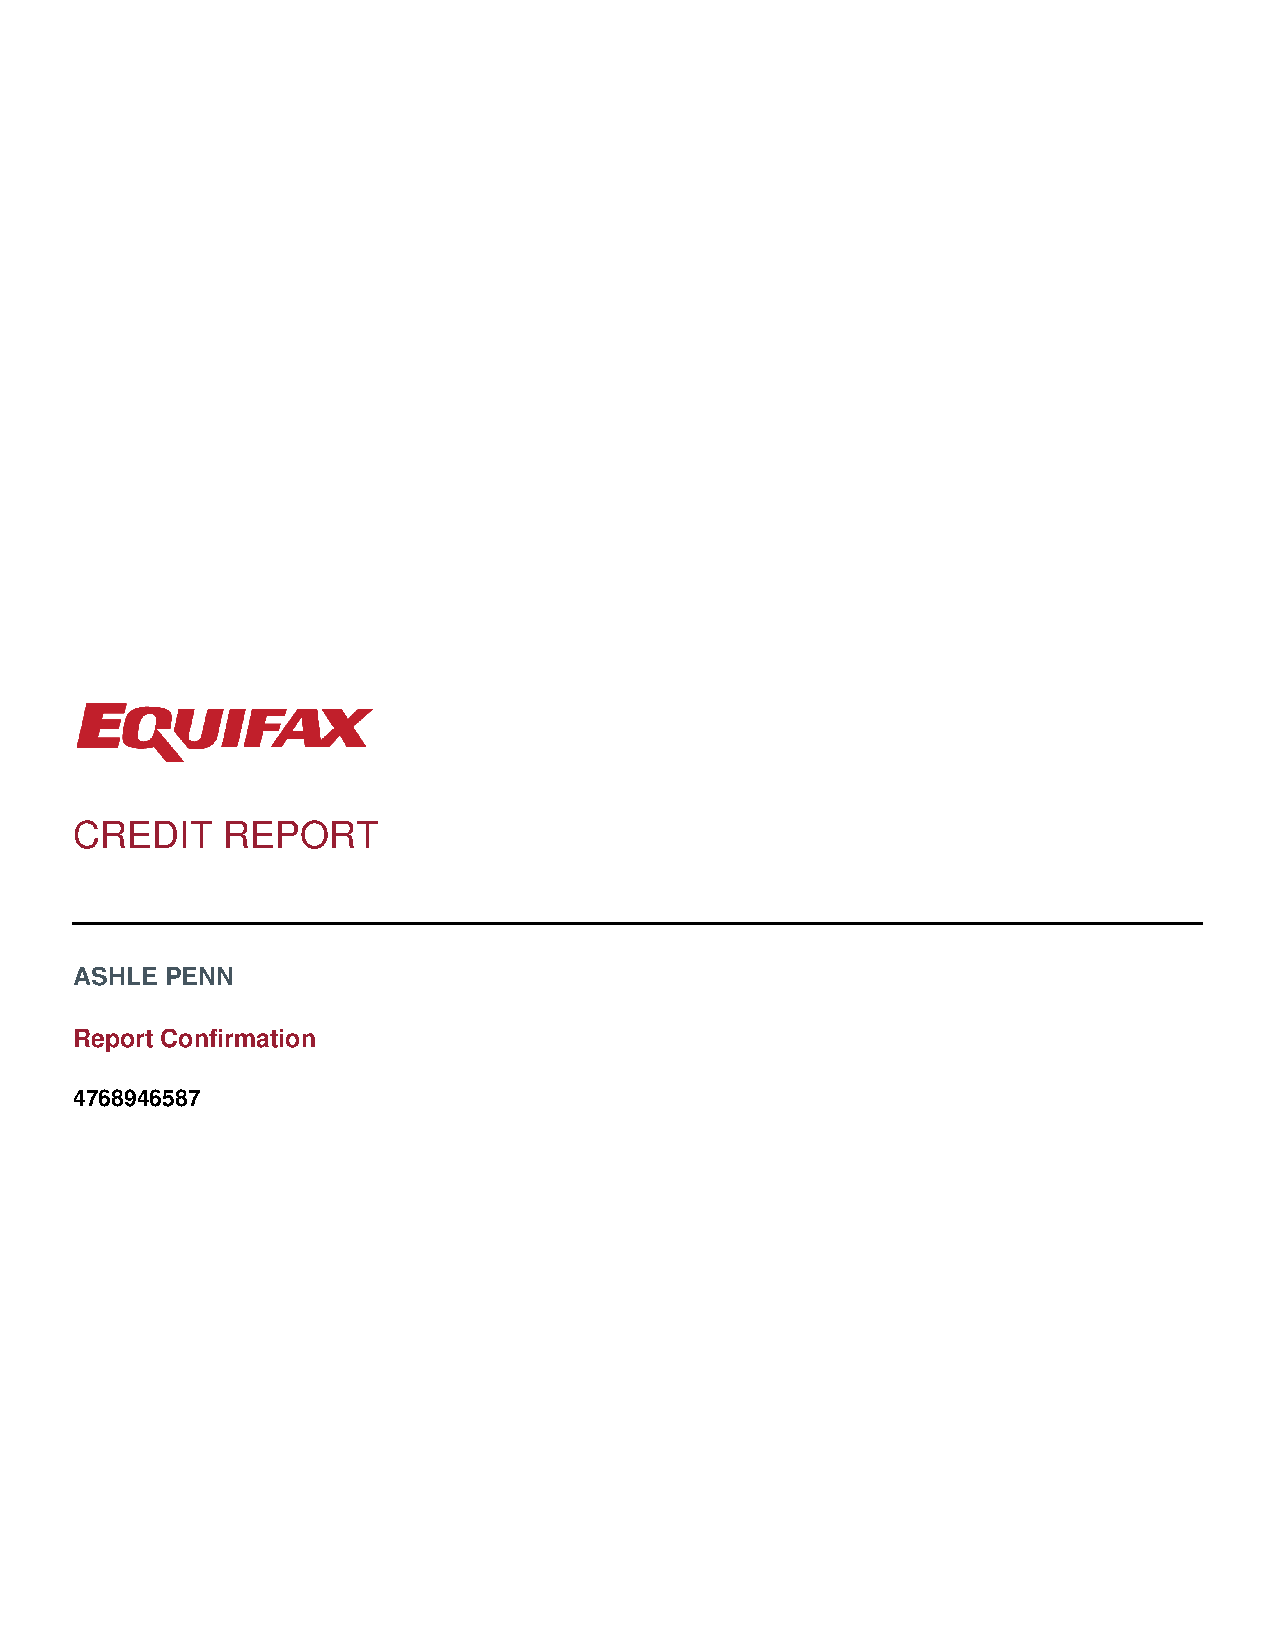
\includepdf[pages=-]{EQUIFAX_9.24.24.pdf}
\newpage \includepdf[pages=-]{EQUIFAX_3.1.26.pdf}
\end{document}
